% 20 Apr 2014 : GWA : 1.5 pages.

\section{Motivation}
\label{sec-motivation}

To better understand storage usage on smartphones and the potential to expand
capacity by creating personal storage clouds, we performed several
measurement studies. We were interested in answering the following questions:

\begin{enumerate}

\item How much storage do users have available on their smartphones?

\item How frequently are media files created, modified, and accessed on
smartphones?

\item How is available storage distributed across multiple personal devices?

\end{enumerate}

Next we discuss our findings and how they influence PocketLocker's design.

\subsection{Rate of Smartphone Storage Decline}

\begin{wraptable}{r}{0.5\textwidth}

\begin{tabularx}{0.5\textwidth}{Xc@{\hspace*{0.1in}}Xc}

\multicolumn{4}{l}{\textbf{By Gender}} \\ \midrule
Female & 127 & Male & 122 \\[0.05in]

\multicolumn{2}{l}{\textbf{By Age}} \\ \midrule
$<$ 18 & 0 & 35--39 & 28 \\
18--20 & 12 & 40--49 & 52 \\
21--24 & 21 & 50--59 & 34 \\
25--29 & 34 & $>$ 60 & 9 \\
30--34 & 35 \\

\end{tabularx}

\caption{\small \textbf{\PhoneLab{} demographic breakdown.}}

\label{table-demographics}

\vspace*{-0.2in}

\end{wraptable}


%\begin{figure}[t]
%
%
\includegraphics[width=\columnwidth]{./figures/single.pdf}
%
%\caption{\small \XXXnote{Storage decline on \PhoneLab{} smartphones.}
%Overall available storage is falling by \XXXnote{XXX~Mb per day} for each
%user, reflecting the rate at which users are generating content and moving
%other files to their mobile devices.}
%
%\label{fig-motivation-decline}
%
%\end{figure}

To determine how rapidly users are creating content on their mobile devices,
we ran an IRB-approved experiment on \PhoneLab{}, a public smartphone testbed
located at the University at Buffalo~\cite{nandugudi2013phonelab}.
288~students, faculty, and staff carry instrumented Android Samsung Galaxy
Nexus smartphones and received subsidized service in return for willingness
to participate in experiments. \PhoneLab{} provides access to a
representative group of smartphone users balanced between genders and drawn
from a wide variety of age brackets, making our results representative of the
broader smartphone user community. Table~\ref{table-demographics} shows a
demographic breakdown of the testbed based on a survey completed by 249 of
the 288 \PhoneLab{} users.

We distributed a simple experiment that periodically logged the storage
available on each smartphone which 105~\PhoneLab{} joined for eight months,
beginning shortly after \PhoneLab{} users received new smartphones in August,
2013. Our log messages show users available storage declining by roughly
30~MB per day, approximately the size of 30~photos or a half-dozen music
files. Aggregate capacity reflects both the rate at which users are creating
content, but also the rate at which they may be moving content such as music
on to their device. However, if this rate of decline continues it will only
take the average \PhoneLab{} participant three years to generate more content
than they can fit onto their Samsung Galaxy Nexus~\cite{galaxynexus} with its
32~GB of Flash. And this estimate shows users coping with the existing
storage limitations of their personal devices. We expect that many already
have far more photos, music, and video than will fit onto their mobile
device.

\subsection{Media Access Patterns}

To obtain a more detailed picture of file access patterns for the media files
that we expect users to want to access on many devices---pictures, movies,
and music---we distributed a second IRB-approved experiment on \PhoneLab{} to
collect more detailed file access patterns. By instrumenting the
\texttt{bionic} C library used by Android applications, we were able to log
every file open performed on all participating devices. We also logged the
file size each time a file was opened. Our changes were distributed as a
platform over-the-air update which \PhoneLab{} participants downloaded in
November, 2013. To indicate consent, participants were also required to
download and run a separate app. We collected one month of data from
December, 2013, for this experiment from 100~users.

\begin{figure}[t]

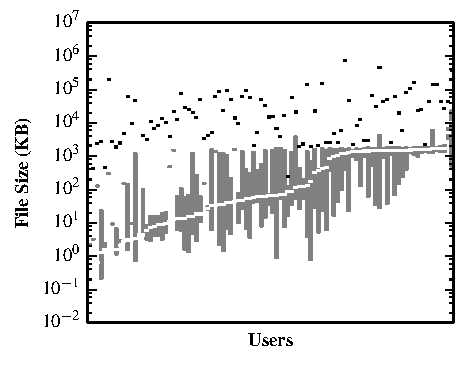
\includegraphics[width=\columnwidth]{./figures/pocketlocker/FileSizeDistributionGraph.pdf}

\caption{\small File Sizes. Per-user distributions are shown for all media
files accessed by \PhoneLab{} users during the one month experiment. Most
files are between 10~KB and 1~MB, but some are up to 100~MB.}

\label{fig-motivation-totals}

\end{figure}

We filtered the dataset by extension to only include media files\footnote{We
marked files with the follow extensions as media: \texttt{flv}, \texttt{mp4},
\texttt{3gp}, \texttt{wmv}, \texttt{avi}, \texttt{mov}, \texttt{mpg},
\texttt{mpeg}, \texttt{aac}, \texttt{jpg}, \texttt{jpeg}, \texttt{png},
\texttt{gif}, \texttt{pdf}, \texttt{bmp}, \texttt{m4a}, \texttt{mp3},
\texttt{m4v}, \texttt{3g2}, \texttt{asf}, \texttt{asx}, \texttt{swp},
\texttt{swf}, and \texttt{tif}.}, which still left \num{1780617} opens of
\num{147756} distinct files by 100~users during the month.
Figure~\ref{fig-motivation-totals} shows CDFs of the total number and size of
the files opened by each \PhoneLab{} user during one month, demonstrating the
smartphone users access a large amount of media content from their mobile
device.

\begin{figure}[t]

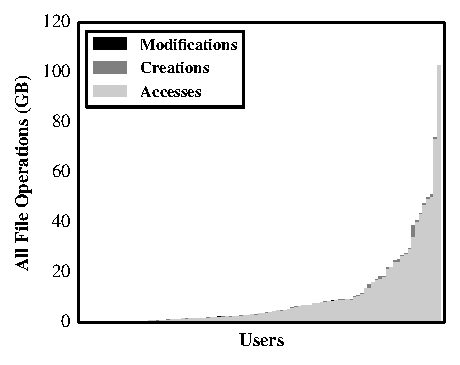
\includegraphics[width=\columnwidth]{./figures/pocketlocker/OperationPercentageGraph.pdf}

\caption{\small \textbf{Media files are rarely modified.} Most file
operations are accesses.}

\label{fig-motivation-modification}

\end{figure}

We marked \num{151904} media files as created if they were empty when opened,
and only \num{11612} files as modified by comparing their sizes reported by
successive open calls. This limited us to files that were opened multiple
times during the trace, but we were still able to determine modifications for
89\% of the file accesses we observed.
Figure~\ref{fig-motivation-modification} shows modifications rates for
photos, video, and audio files, demonstrating that these files are rarely
modified on mobile devices. PocketLocker incorporates this assumption into
its design.

\subsection{Available Storage Distribution}

\begin{table}[t]
{\small

\begin{tabularx}{\columnwidth}{Xccc}

\textbf{Location} & \textbf{Min~(GB)} & \textbf{Mean~(GB)} &
\textbf{Max~(GB)} \\ \toprule
Home & 8 & 308 & 3000 \\
Work & 7 & 97 & 600 \\
Mobile & 0.5 & 10 & 42 \\
Total & 15 & 415 & 3806 \\

\end{tabularx}
}

\caption{\small \textbf{Storage space available at different locations.}
Results from a survey of 47 people. Users have an order-of-magnitude less
space available on mobile devices compared with their other personal
devices.}

\label{table-storagesurvey}

\end{table}

Finally, to investigate the potential to utilize other nearby personal
devices as part of a personal storage cloud, we distributed an IRB-approved
survey to undergraduates at our university. For each device they owned,
respondents were asked to indicate how much storage capacity it had available
and, for immobile devices, where they used it most: at work or school, or at
home. Table~\ref{table-storagesurvey} shows results collected from 47
volunteers. Results indicate that users have large storage capacity from
other devices, such as laptops and desktops, available to them at multiple
locations, while the free storage available on their smartphones was one
order-of-magnitude smaller than the storage available on their other devices.
By utilizing storage on other personal devices, PocketLocker can address the
mobile storage bottleneck.
